\chapter{Data survey}

\section{Dataset}
In this research, the dataset was collected via a structured survey on the SurveyMonkey platform to understand elderly participants' needs and expectations from the medical assistive robot, Medora. A total of around sixty to sixty-five respondents, both male and female over the age of sixty, participated. The dataset captures respondents' prior exposure to assistive robots, interest in adoption, and opinions on advanced features such as facial and emotional recognition. It also includes their comfort with multilingual communication, expectations regarding cost and emergency support, and concerns or challenges they foresee in using such a system. Both closed- and open-ended questions were used, allowing collection of both quantitative trends and qualitative insights. This resulted in a rich dataset that reflects the perspectives of the elderly population, ensuring that findings are grounded in real user needs.

\subsection{Implications of This Dataset on Our Research}
The dataset is essential as it provides a user-centered foundation for Medora’s design. For example, over 80\% of participants had never heard of a health-assistive robot, highlighting the importance of simplicity and intuitive use. Similarly, 71\% believed Medora could help reduce loneliness, reinforcing the value of emotional interaction and communication features. Preferences for reminders, SOS alerts, and bilingual support were strong, while price sensitivity and privacy concerns emerged as critical barriers. Altogether, these insights guided us in shaping Medora to be both functional and acceptable for its intended users.


\section{Survey and Interview Process}

The survey and interview process was designed to meet the needs of the senior population. A detailed questionnaire was first drafted, tested with a pilot group for clarity, and refined accordingly. The final survey was distributed via SurveyMonkey, with both online and in-person support to ensure inclusivity. Semi-structured interviews were also conducted, encouraging participants to elaborate on their preferences, concerns, and expectations. Given that many had no prior experience with robotic technologies, it was essential to create a comfortable and respectful environment. Overall, this process enabled us to capture both quantitative data and rich qualitative insights.

\subsection{Interview and Survey Goals}

The primary goal of the surveys and interviews was to gather actionable information so Medora’s design aligned with real user needs. The survey measured perceptions of robot assistance, desirable features, and potential barriers, while interviews added context by uncovering why participants considered certain features essential or problematic. For example, questions explored willingness to use robots in different languages, expectations of emergency functions, and privacy concerns. This combination went beyond data collection to build a more empathic understanding of elderly users.

\subsection{Participants and Data Collection}

Participants were elderly individuals aged 60 and above, representing diverse backgrounds and equally including men and women. This demographic was chosen as they are the primary beneficiaries of health-assistive robots. Data was collected both online (via SurveyMonkey) and in person to accommodate digital accessibility concerns. Anonymity and participant comfort were prioritized, ensuring honest and representative responses.

\subsection{Survey and Interview Designs}

Following human-centered design principles, the survey consisted of sections regarding familiarity with robotics, intended use of Medora, evaluation of various features, and open-ended feedback. In addition to providing quantitative data in the multiple-choice questions, the open-ended questions provided participants' individual perspectives. Each interview was semi-structured, prompting participants; however, participants narrated their daily routines, comes expectations, and concerns. Small informal dimensions either in person or on a video call enabled participants to interact comfortably. The semi-structured nature of the interview provided more formulated, fuller discussions around the features such as facial recognition, privacy concerns, and forced autonomy, providing context to survey responses.

\textbf{Preferences:}The survey results show respondents’ priorities were on practical functions like medication reminders, SOS alerts, and health monitoring. They also appreciated the interactive features like emotion and facial recognition, which are aspects of Medora that gave it a more human feel. Many of the respondents stressed auditory communication (voice reminders) was essential because they have difficulty reading notifications or complex menus.

\textbf{Expected Role:} Survey respondents imagined Medora as an active participant instead of a passive device—overseeing vital sign monitoring and reminding users of medication schedules, as well as reaching out to family members or doctors in an emergency. Beyond the caregivers’ role, 71\% of respondents also expected Medora to help alleviate loneliness, emphasizing the device’s dual purpose as an aide and a companion.



\subsection{Essential Steps of the Survey}

The research process involved three stages: (1) preparation—drafting and piloting the questionnaire; (2) data collection—distributing surveys online and in person while ensuring completeness and accuracy; and (3) reporting—exporting responses into structured formats  for analysis. Each stage was vital to ensure reliability and representativeness.

\subsection{The Importance of Surveys and Interviews}

Surveys and interviews were crucial to demonstrating that Medora’s design was driven by real needs not assumptions. Surveys can identify measurable trends, such as preferences for voice reminders and sensitivity to price, while accompanying interviews helped us better understand the underlying challenges such as not being able to read reminders or use complex software. Ultimately, surveys and interviews showed us that Medora must be imagined as more than just a tangible tool, but also as a friend who is able to empathize with the needs of older adults.
 advanced. advanced.

\section{Survey Questionnaire}
We used a survey questionnaire to capture multiple aspects of elderly care robotics, including prior exposure to health-assistive robots, interest in using Medora, and opinions about core features like facial recognition, emotional detection, and language preferences. We also asked about desired functions, emergency contacts, and ease of use. In the open-ended section of the survey, we invited participants to provide ideas for additional features in Medora, giving us qualitative insights to support the quantitative analyses.

\subsection{Demographic Data}

The participants were older adults, ages 60-75, male and female, mostly retired or partially retired, living alone or with family. This demographic is relevant with respect to their medical need for reminders, emotional support, and health monitoring. The participants in this group never used a health-assistive robot, however, many were excited and open to using new technology. The sample also reflected both urban and semi-urban locations, making real-world considerations for a diverse representation of elderly needs and expectations.

\subsection{Preference for Robot and Features}
Survey results showed a strong interest in Medora. Respondents expressed trust, reliability, and user-friendliness were most important to them. The majority of interested users also indicated a preference for facial recognition, emotion detection, and being able to switch languages. As a whole, respondents indicated a preference for Bangla, however many preferred a bilingual Bangla-English version. Most respondents placed significant emphasis on ease of interaction without the use of screens by way of voice communication with Medora. Respondents described reliability, accuracy, and continuous operating behavior as their core expectations for Medora.

\subsection{Functionality, Rules, and Personality}

Participants would expect Medora to have core functionality, including reminding someone to take their medications, monitoring vital signs, and sending an SOS alert to family members. They also mentioned the ability to responsively recognize emotions and moods, specifically when someone was feeling sad, stressed, or needed social interaction. Data privacy and how Medora would keep personal information safe were recurring issues, as well as providing easy controls to allow for independent user engagement. For personality, respondents expressed favouritism towards a polite, calm, and encouraging tone that was consistent each interaction, as well as someone who was friendly and could gain trust in their daily interactions.
\section{ Survey Response Data}

\subsection{Pre-Survey}
The pre-survey for elderly care assistive robots is an important first step because it records user demographics, lifestyle, and level of comfort with technology. These data inform the design of sensing, interaction, and system usability according to actual needs. The survey highlights healthcare gaps such as medication adherence, trust in robotic support, preferred interaction modes, and psychosocial components (e.g., reducing loneliness). Data-driven insights from the pre-survey enable decision-making for system features, adoption strategies, and meaningful impact in elderly care.

\begin{enumerate}
    \item \textbf{Mapping age group in surveyed family (Under 20 / 20--40 / 41--60 / 61+)}  
    Age demographics show a variety of participants. A larger percentage in the 61+ group demonstrates the core elderly population as primary beneficiaries. Younger age groups provide caregiver/family perspectives important for adoption.  
    \begin{figure}[H]
        \centering
        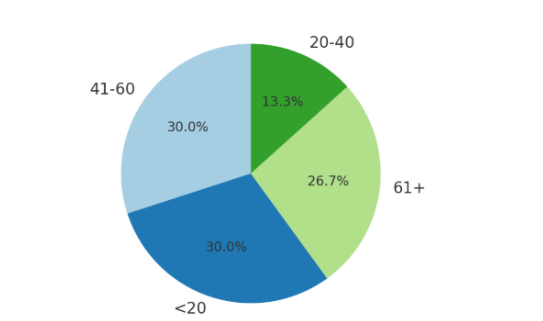
\includegraphics[width=0.5\textwidth]{Medora_thesis (1)/pics/thesis/Slide Shows/1.png}
        \caption{Mapping age group of surveyed family members}
    \end{figure}

    \item \textbf{Living arrangement (Alone / With family)}  
    Living arrangements determine care needs. A higher percentage of ``alone'' responses signals greater need for safety and companionship, while living with family frames the robot as a supplemental tool.  
    \begin{figure}[H]
        \centering
        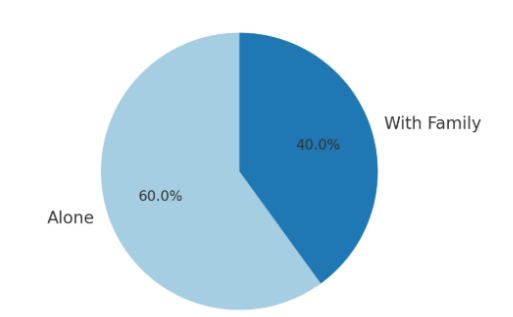
\includegraphics[width=0.4\textwidth]{Medora_thesis (1)/pics/thesis/Slide Shows/2.png}
        \caption{Rate of elderly people alone during working hours}
    \end{figure}

    \item \textbf{Have you used a healthcare robot before? (Yes/No)}  
    Responses reveal awareness. A low ``Yes'' percentage highlights the need for user-friendly, first-time experiences. A higher ``Yes'' shows readiness for adoption.  
    \begin{figure}[H]
        \centering
        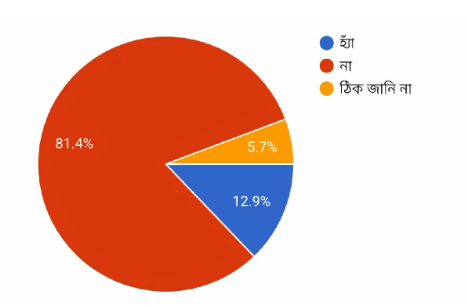
\includegraphics[width=0.4\textwidth]{Medora_thesis (1)/pics/thesis/Slide Shows/3.png}
        \caption{Prior use of healthcare robots}
    \end{figure}

    \item \textbf{Comfort with technology (Likert scale: Very Uncomfortable $\rightarrow$ Very Comfortable)}  
    Responses show variation in comfort. Uncomfortable users require simple voice-first design, while comfortable users are ready for advanced IoT integration.  
    \begin{figure}[H]
        \centering
        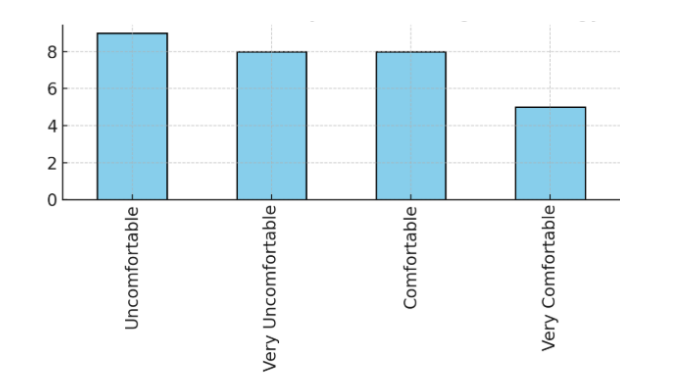
\includegraphics[width=0.4\textwidth]{Medora_thesis (1)/pics/thesis/Slide Shows/4.png}
        \caption{Comfort with technology in daily life}
    \end{figure}

    \item \textbf{How often do you forget to take medicine? (Never / Sometimes / Often / Always)}  
    Responses indicate medication adherence issues. High ``Sometimes/Often'' percentages justify reminder functionality.  
    \begin{figure}[H]
        \centering
        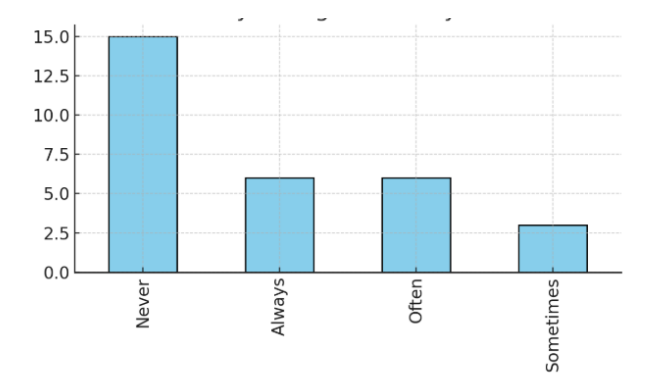
\includegraphics[width=0.6\textwidth]{Medora_thesis (1)/pics/thesis/Slide Shows/5.png}
        \caption{Forgetting to take medicine}
    \end{figure}

    \item \textbf{How often do you use smart devices? (Never / Occasionally / Daily / Multiple times daily)}  
    Daily/multiple usage indicates familiarity with smart devices, while low usage requires intuitive design.  
    \begin{figure}[H]
        \centering
        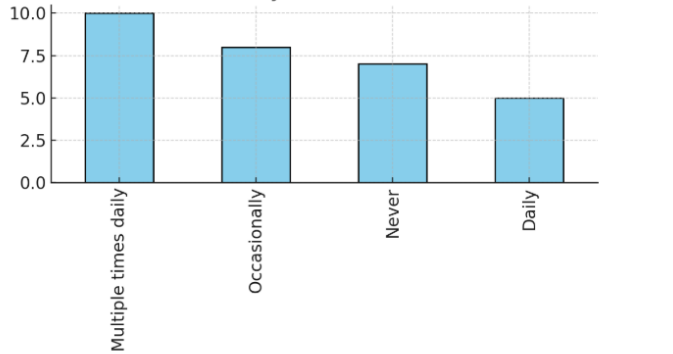
\includegraphics[width=0.6\textwidth]{Medora_thesis (1)/pics/thesis/Slide Shows/6.png}
        \caption{Use of smart devices among respondents}
    \end{figure}

    \item \textbf{Trust in robot reminders (Yes / No / Not sure)}  
    Responses reflect willingness to trust robotic reminders. ``Not sure'' signals hesitance requiring awareness campaigns.  
    \begin{figure}[H]
        \centering
        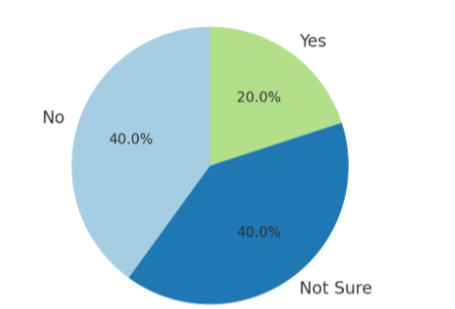
\includegraphics[width=0.4\textwidth]{Medora_thesis (1)/pics/thesis/Slide Shows/7.png}
        \caption{Trust in robots for medication reminders}
    \end{figure}

    \item \textbf{Preferred mode of receiving reminders}  
    Majority (60\%) preferred auditory prompts, followed by mobile notifications (27.14\%), on-screen prompts (10\%), and SMS (2.86\%).  
    \begin{figure}[H]
        \centering
        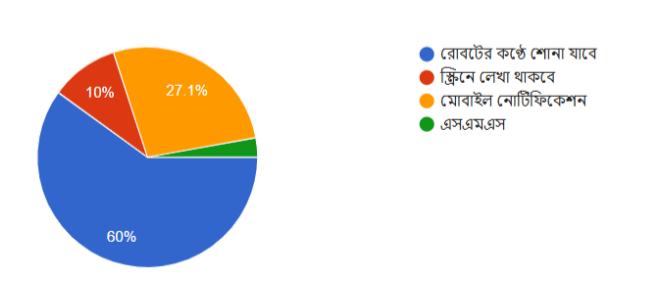
\includegraphics[width=0.7\textwidth]{Medora_thesis (1)/pics/thesis/Slide Shows/8.png}
        \caption{Preferred mode of reminders}
    \end{figure}

    \item \textbf{Belief about Medora’s potential to reduce loneliness}  
    71.43\% believe the robot can serve as both assistant and companion.  
    \begin{figure}[H]
        \centering
        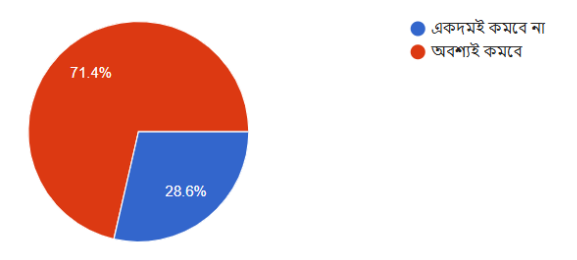
\includegraphics[width=0.6\textwidth]{Medora_thesis (1)/pics/thesis/Slide Shows/9.png}
        \caption{Belief in Medora reducing loneliness}
    \end{figure}
\end{enumerate}

\subsection{Post-Survey}
The post-survey was conducted after introducing Medora’s features to the participants. It aimed to capture changes in perceptions and acceptance.

\begin{enumerate}
    \item \textbf{Interest in using Medora}  
    24.29\% very interested, 31.43\% interested, 32.86\% neutral, 7.14\% low interest, 4.29\% no interest.  
    \begin{figure}[H]
        \centering
        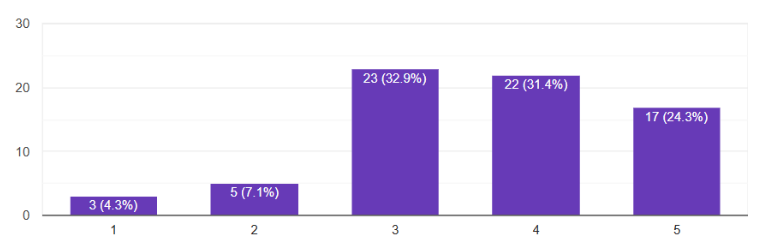
\includegraphics[width=0.6\textwidth]{Medora_thesis (1)/pics/thesis/Slide Shows/10.png}
        \caption{Interest level in using Medora}
    \end{figure}

    \item \textbf{Importance of facial recognition}  
    34.29\% very necessary, 24.29\% necessary, 30\% neutral, 7.14\% less necessary, 4.29\% not necessary.  
    \begin{figure}[H]
        \centering
        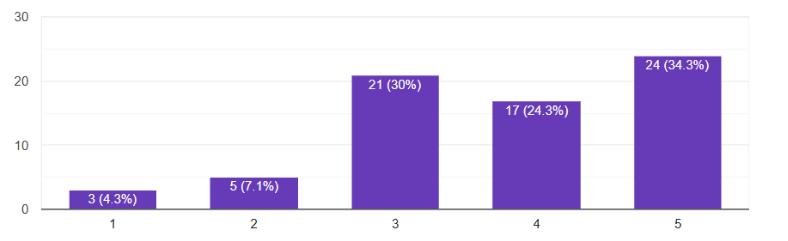
\includegraphics[width=0.6\textwidth]{Medora_thesis (1)/pics/thesis/Slide Shows/11.png}
        \caption{Importance of facial recognition}
    \end{figure}

    \item \textbf{Usefulness of emotion understanding}  
    45.71\% very useful, 32.86\% moderately useful, 11.43\% not useful, 10\% no opinion.  
    \begin{figure}[H]
        \centering
        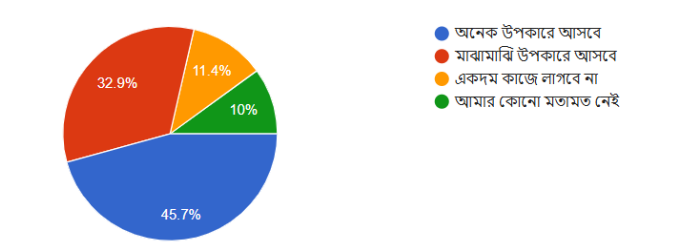
\includegraphics[width=0.6\textwidth]{Medora_thesis (1)/pics/thesis/Slide Shows/12.png}
        \caption{Usefulness of emotion recognition}
    \end{figure}

    \item \textbf{Most important features in Medora}  
    24.29\% selected multiple functions (reminders, temp, face/emotion detection, SOS). Other responses varied across simpler combinations.  
    \begin{figure}[H]
        \centering
        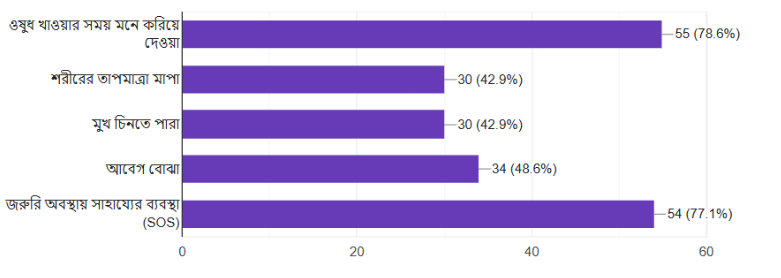
\includegraphics[width=0.6\textwidth]{Medora_thesis (1)/pics/thesis/Slide Shows/13.png}
        \caption{Key features considered most important}
    \end{figure}

    \item \textbf{Preferred interaction language}  
    45.71\% Bangla, 41.43\% bilingual, 12.86\% English.  
    \begin{figure}[H]
        \centering
        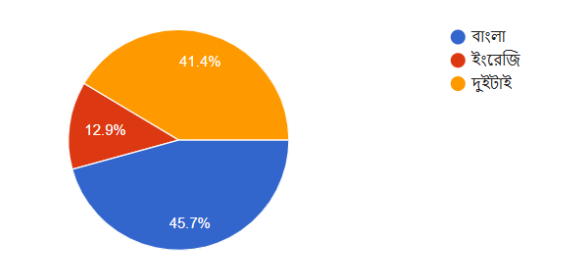
\includegraphics[width=0.6\textwidth]{Medora_thesis (1)/pics/thesis/Slide Shows/14.png}
        \caption{Preferred interaction language}
    \end{figure}

    \item \textbf{Main concerns with Medora}  
    Concerns included learning (17.14\%), privacy (15.71\%), performance (12.86\%), no concern (12.86\%). Others mentioned cost and reliability.  
    \begin{figure}[H]
        \centering
        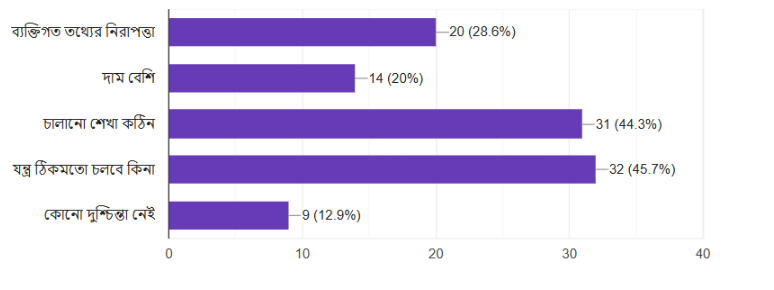
\includegraphics[width=0.6\textwidth]{Medora_thesis (1)/pics/thesis/Slide Shows/15.png}
        \caption{Main concerns regarding Medora}
    \end{figure}

    \item \textbf{Comfort level using Medora}  
    44.29\% neutral, 27.14\% comfortable, 14.29\% very comfortable, 11.43\% slightly uncomfortable, 2.86\% very uncomfortable.  
    \begin{figure}[H]
        \centering
        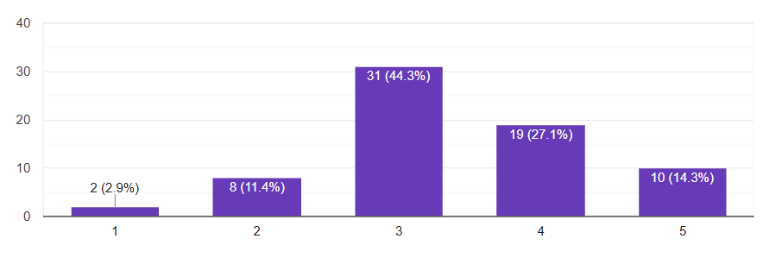
\includegraphics[width=0.6\textwidth]{Medora_thesis (1)/pics/thesis/Slide Shows/16.png}
        \caption{Comfort level in using Medora}
    \end{figure}

    \item \textbf{Acceptable price range}  
    47.14\% prefer 10,000–20,000 BDT, 25.71\% under 10,000 BDT, 27.14\% between 20,000–30,000 BDT.  
    \begin{figure}[H]
        \centering
        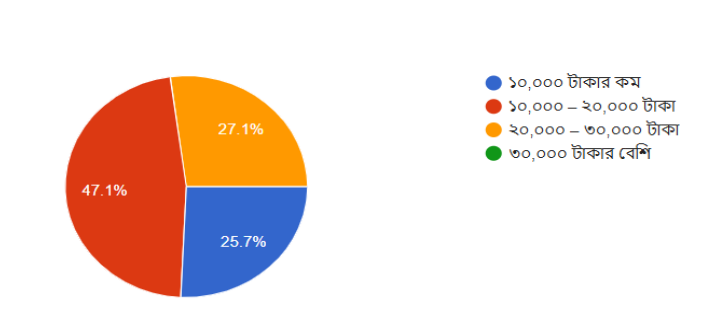
\includegraphics[width=0.6\textwidth]{Medora_thesis (1)/pics/thesis/Slide Shows/17.png}
        \caption{Preferred price range for Medora}
    \end{figure}

    \item \textbf{Preferred recipients of emergency alerts}  
    78.57\% family, 12.86\% hospital helpline, 5.71\% doctor, 2.86\% neighbours.  
    \begin{figure}[H]
        \centering
        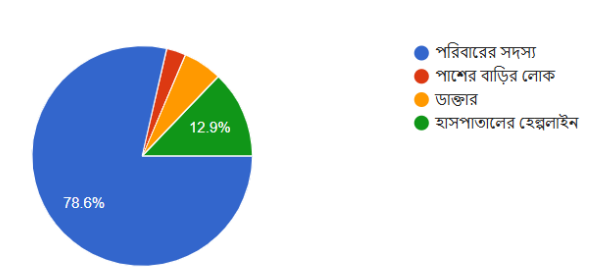
\includegraphics[width=0.6\textwidth]{Medora_thesis (1)/pics/thesis/Slide Shows/18.png}
        \caption{Preferred emergency alert recipients}
    \end{figure}

    \item \textbf{Most appreciated aspect of Medora}  
    Responses varied: 21.43\% health+tech, 18.57\% health only, 15.71\% all features, 14.29\% tech only.  
    \begin{figure}[H]
        \centering
        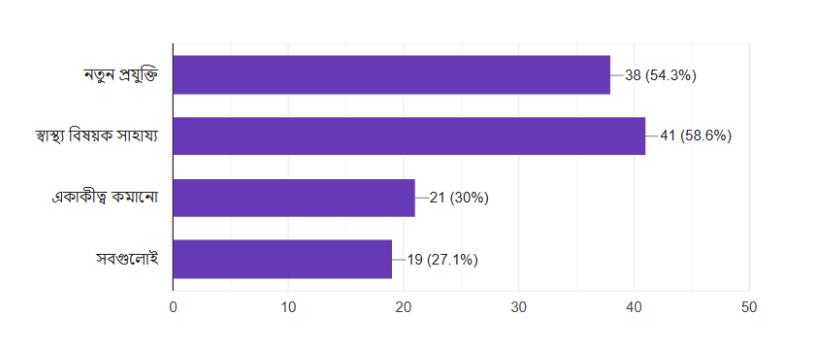
\includegraphics[width=0.6\textwidth]{Medora_thesis (1)/pics/thesis/Slide Shows/19.png}
        \caption{Most appreciated aspect of Medora}
    \end{figure}

    \item \textbf{Assistance needed to operate Medora}  
    42.86\% may need help, 34.29\% independent, 22.86\% certain they need help.  
    \begin{figure}[H]
        \centering
        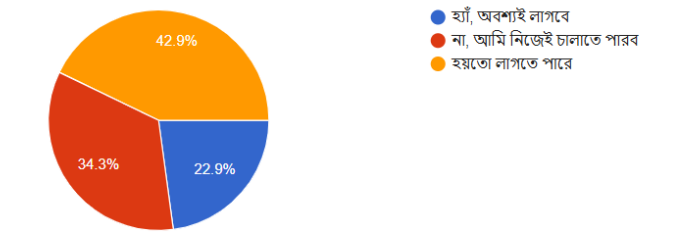
\includegraphics[width=0.6\textwidth]{Medora_thesis (1)/pics/thesis/Slide Shows/20.png}
        \caption{Assistance required to operate Medora}
    \end{figure}

    \item \textbf{Additional comments and suggestions}  
    Participants mentioned: \textit{``Very helpful''}, \textit{``Good initiative''}, \textit{``Should be affordable''}, \textit{``Ensure data security''}. These reflect improvement directions in affordability, reliability, and trustworthiness.
\end{enumerate}


\begin{table}[H]
\centering
\caption{Pre- and Post-Survey Findings}
\renewcommand{\arraystretch}{1.3} % increases row height
\begin{tabularx}{\textwidth}{|>{\raggedright\arraybackslash}p{3cm}|X|X|}
\hline
\textbf{Category} & \textbf{Pre-Survey Findings} & \textbf{Post-Survey Findings} \\
\hline
\textbf{Demographics} & Majority above 61 years; mix of living alone and with family & Same population; more openness to technology reported \\
\hline
\textbf{Experience with Robots} & Limited or no prior experience & Increased interest after hands-on interaction \\
\hline
\textbf{Comfort with Technology} & Mostly low to moderate comfort & Notable improvement; majority neutral to positive \\
\hline
\textbf{Medication Habits} & Frequent forgetting of medication reported & Positive response to reminder functionality (24.29\% highly useful) \\
\hline
\textbf{Trust in Robots} & Mostly undecided & Over half (56\%) showed interest in continued use \\
\hline
\textbf{Loneliness Reduction} & 70\% believed robots could help reduce loneliness & Acceptance strengthened after use \\
\hline
\textbf{Preferred Reminders} & 60\% auditory, followed by mobile and visual prompts & Auditory reminders confirmed as most effective \\
\hline
\textbf{Key Features} & Anticipated reminders and interaction & Emotion recognition (78.57\%), facial recognition (58.58\%), bilingual support (87\%) rated highly useful \\
\hline
\textbf{Concerns} & Uncertainty about trust and adaptability & Learning needs (17.14\%), privacy risks (15.71\%), and performance reliability (12.86\%) remained concerns \\
\hline
\textbf{User Ratings} & N/A & Overall user satisfaction: ★★★★☆ (4/5 stars) \\
\hline
\end{tabularx}
\end{table}


\begin{figure}[H]
    \centering
    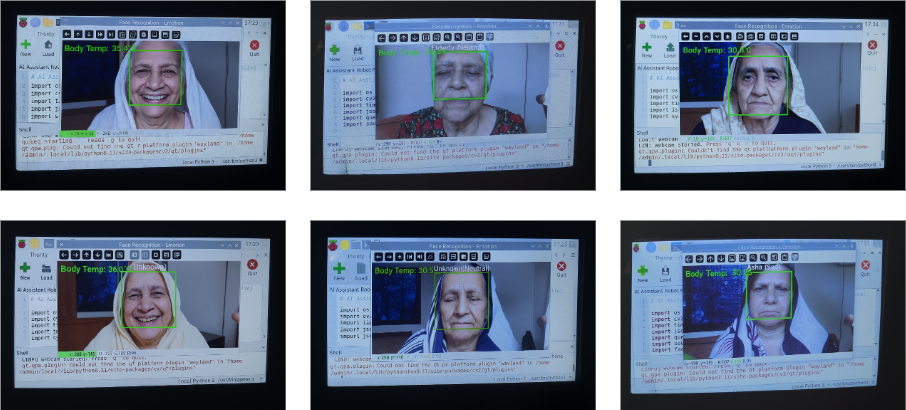
\includegraphics[width=0.7\textwidth]{Medora_thesis (1)/pics/thesis/Untitled Diagram.drawio (1).png}
    \caption{Participants who interacted with Medora and provided feedback}
    \label{fig:users}
\end{figure}
